\documentclass[tikz,border=10pt]{standalone}
\usepackage{pgfplots}
\pgfplotsset{compat=1.16}

\begin{document}
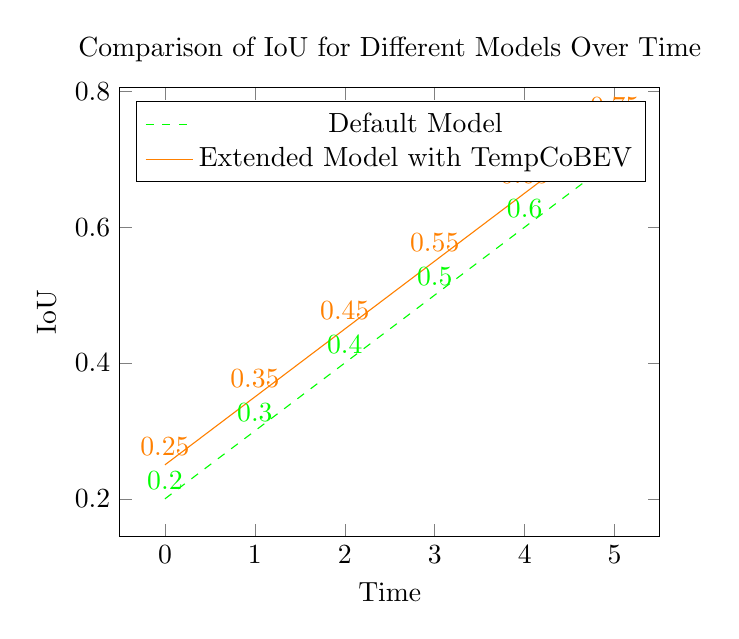
\begin{tikzpicture}
    \begin{axis}[
        title={Comparison of IoU for Different Models Over Time},
        xlabel={Time},
        ylabel={IoU},
        legend pos=north west,
        xtick=data,
        nodes near coords,
        nodes near coords align={vertical},
        ]
        
        % Default Model - Green Dashed Line
        \addplot[green,dashed] coordinates {
            (0, 0.2)
            (1, 0.3)
            (2, 0.4)
            (3, 0.5)
            (4, 0.6)
            (5, 0.7)
            };
        \label{default-model}
        
        % Extended Model with TempCoBEV - Orange Solid Line
        \addplot[orange,solid] coordinates {
            (0, 0.25)
            (1, 0.35)
            (2, 0.45)
            (3, 0.55)
            (4, 0.65)
            (5, 0.75)
            };
        \label{tempcobev-model}
        
        % Legend Entries
        \legend{Default Model, Extended Model with TempCoBEV}
    \end{axis}
\end{tikzpicture}
\end{document}